\documentclass[a4paper, 12pt]{article} % тип документа

%%%Библиотеки
	%\usepackage[warn]{mathtext}	
	\usepackage[T2A]{fontenc}   %Кодировка
	\usepackage[utf8]{inputenc} %Кодировка исходного текста
	\usepackage[english, russian]{babel} %Локализация и переносы
	\usepackage{caption}
	\usepackage{listings}
	\usepackage{amsmath, amsfonts, amssymb, amsthm, mathtools}
	\usepackage[warn]{mathtext}
	\usepackage[mathscr]{eucal}
	\usepackage{wasysym}
	\usepackage{graphicx} %Вставка картинок правильная
	\DeclareGraphicsExtensions{.pdf,.png,.jpg}
	\graphicspath{ {images/} }
	
	\setlength{\parskip}{0.5cm}
	
	\usepackage{pgfplots}
	\usepackage{indentfirst}
	\usepackage{float}    %Плавающие картинки
	\usepackage{wrapfig}  %Обтекание фигур (таблиц, картинок и прочего)
	\usepackage{fancyhdr} %Загрузим пакет
	\usepackage{lscape}
	\usepackage{xcolor}
	\usepackage[normalem]{ulem}
	\usepackage{wasysym}
	\usepackage{subfig}
	\usepackage{graphicx}
	
	\usepackage{titlesec}
	\titlelabel{\thetitle.\quad}

	\usepackage{hyperref}
	\newenvironment{comment}{}{}

%%%Конец библиотек

%%%Настройка ссылок
%%%	\hypersetup
%%%	{
%%%		colorlinks = true,
%%%		linkcolor  = blue,
%%%		filecolor  = magenta,
%%%		urlcolor   = blue
%%%	}
%%%Конец настройки ссылок


%%%Настройка колонтитулы
    \pagestyle{fancy}
    \fancyhead{}
    \fancyhead[L]{1.1.1}
    \fancyhead[R]{Засимов Георгий, группа Б01-109}
    \fancyfoot[C]{\thepage}
%%%конец настройки колонтитулы



\begin{document}
                        %%%%Начало документа%%%%


%%%Начало титульника
\begin{titlepage}

    \newpage
    \begin{center}
        \normalsize Московский физико-технический институт \\(национальный исследовательский университет)
    \end{center}

    \vspace{6em}

    \begin{center}
        \Large Лабораторная работа по общему курсу физики\\
    \end{center}

    \vspace{1em}

    \begin{center}
        \Large \textbf{1.1.1. Определение систематических и случайных погрешностей при измерении удельного сопротивления нихромовой проволки}
    \end{center}

    \vspace{2em}

    \begin{center}
        \large Засимов Георгий Алексеевич \\
        Группа Б01-109
    \end{center}

    \vspace{\fill}

    \begin{center}
    Долгопрудный \\2021
    \end{center}
    
\end{titlepage}
%%%Конец Титульника


%%%%Настройка оглавления и нумерации страниц
    \thispagestyle{empty}
    \newpage
    \tableofcontents
    \newpage
    \setcounter{page}{1}
%%%%Настройка оглавления и нумерации страниц

\section{Аннотация}

\textbf{Цель работы:} измерить удельное сопротивление проволоки и вычислить систематические и случайные погрешности при использовании таких измерительных приборов, как линейка, штангенциркуль, микрометр, амперметр, вольтметр и мост постоянного тока.\\

\textbf{Используемое оборудование:} линейка, штангенциркуль, микрометр, отрезок проволоки из нихрома, амперметр, вольтметр, источник ЭДС, мост постоянного тока, реостат, ключ.\\

\textbf{Используются следующие методы измерений сопротивления:} 

1) Определение углового коэффициента наклона зависимости напряжения на проволоке от тока через неё, измеряемых с помощью аналоговых и цифровых вольтметров и амперметров.

2) Измерение с помощью моста постоянного тока. Геометрические размеры образца измеряются с помощью линейки, штангенциркуля и микрометра. Детально исследуется систематические и случайные погрешности проводимых измерений.

В данной работе мы используем оба метода и сравниваем их.\\


\section{Теоретические сведения}

Удельное сопротивленеи проволоки круглого сечения, изготовленного из однородного материала и имеющей всюду одинаковую толщину, может быть определено по формуле
\[\rho = \frac{R_{\text{пр}}}{L} \frac{\pi d^2}{4}\]

В этой формуле $R$ -- сопротивление измеряемого отрезка проволоки, $d$ -- диаметр проволоки, $L$ -- длина отрезка проволоки.

Так как диаметр проволоки флуктуирует в зависимости от места измерения и толщины, необходимо найти среднее значение толщины по всей длине проволоки. Также необходимо учесть погрешность измеренной средней толщины при подсчёте погрешности удельного сопротивления проволоки.

Сопротивление проволоки можно искать с помощью двух различных (очень схожих) электрических схем:
\begin{center}
    {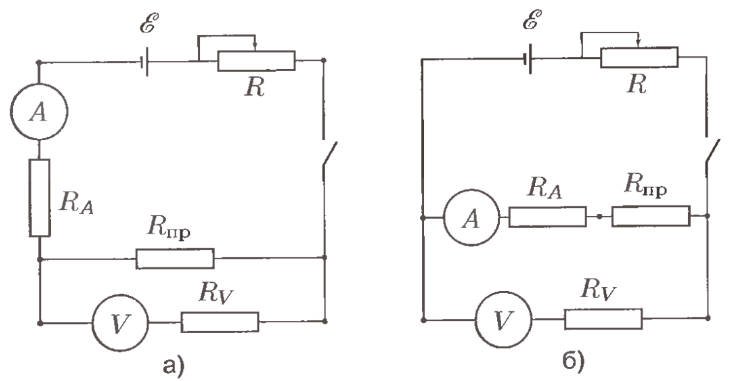
\includegraphics[width=11cm]{1}}
\end{center}

На данных схемах $R_V$ и $R_A$ -- сопротивления вольтметра и амперметра соответственно, а $R$ -- сопротивление реостата.

Для схемы a) имеем:
\[R_{\text{пр1}} = \frac{V_a}{I_a} = R_{\text{пр}} \frac{R_V}{R_V + R_{\text{пр}}} \]

Здесь $R_{\text{пр1}}$ -- измеренное сопротивление проволоки по закону Ома без учёта конечности сопротивления вольметра.

Для схемы б) имеем:
\[R_{\text{пр2}} = \frac{V_{\text{б}}}{I_{\text{б}}} = R_{\text{пр}} + R_A\]

Здесь $R_{\text{пр2}}$ -- измеренное сопротивление проволоки по закону Ома без учёта того, что у амперметра есть сопротивление.

Преобразуем оба выражения:
\[R_{\text{пр}} = R_{\text{пр1}} \frac{R_V}{R_V - R_{\text{пр1}}} = \frac{R_{\text{пр1}}}{1 - (R_{\text{пр1}})/(R_V)} \cong R_{\text{пр1}} (1 + \frac{R_{\text{пр1}}}{R_V})\]

\[R_{\text{пр}} = R_{\text{пр1}} (1 - \frac{R_A}{R_{\text{пр2}}})\]

Естественно, использовтаь надо то выражение, которое даёт меньшую поправку на сопротивление.\\

\section {Оборудование и инструментальные погрешности}


\textbf{Линейка:} $\vartriangle_{лин} = 0,5$ мм (по цене деления). При определении положений контактов имеется дополнительная погрешность, которая может быть оценена как  $\vartriangle_{лин} = \pm2$ мм.\\
\textbf{Штангенциркуль:} $\vartriangle_{шт} = 0,1$ мм (маркировка производителя).\\
\textbf{Микрометр:} $\vartriangle_{мкм} = 0,01$ мм (маркировка производителя).\\
\textbf{Вольтметр:} погрешность измерения вольтметра вычисляется согласно паспорту устройства для используемого напряжения 5В по формуле: $\vartriangle_{вм} = \pm(0,0003 X + 4 k)$ мВ , где X -- полученное значение напряжения, k -- порядок полученного измерения.\\
\textbf{Амперметр:} при измерниях в диапазоне 20 мА до 300 мА погрешность амперметра составила 0,5\%. \\


В диапазоне измерения R от 1 до 10 Ом относительная поправка $\frac{R'}{R_{V}}$ к сопротивлению согласно формуле \eqref{сопр образца} составляет от 0,01\% (при R = 1 Oм и $R_{V}$ 10 кОм) до 0,2\% (при R 10 Ом и
$R_{V}$ кОм). Следовательно, данная поправка заведомо меньше погрешности измерений (0,5\% для вольтметра), поэтому примем далее, что неидеальность вольтметра не оказывает влияния на измерение сопротивления:   $R \approx R'$\\


\textbf{Мост постоянного тока Р4833:}\\
Класс точности: 0,1\\
Разрядность магазина сопротивлений: 5 ед.\\
Используемый диапазон измерений: 10−4 – 10 Ом (для множителя $N = 10^2$).
Погрешность измерений в используемом диапазоне: ±0,010 Ом.


\newpage

\section{Результаты измерений диаметра проволоки}


Составим таблицу на основе измеренных данных толщины проволоки с помощью штангенциркуля и микрометра:

\begin{center}
\begin{tabular}{|c|c|c|c|c|c|c|c|c|c|c|}
\hline 
 & 1 & 2 & 3 & 4 & 5 & 6 & 7 & 8  \\ 
\hline 
$d_{10},$ мм & 0,4 & 0,4 & 0,4 & 0,4 & 0,4 & 0,4 & 0,4 & 0,4\\ 
\hline 
$d_{20},$ мм & 0,36 & 0,36 & 0,37 & 0,37 & 0,36 & 0,35 & 0,35 & 0,36\\ 
\hline 
\end{tabular} 
\end{center}

При измерении диаметра проволоки штангенциркулем случайная погрешность измерений отсутствует. Следовательно, точность результата определяется только точностью штангенциркуля (систематической погрешностью):
\[d_{10} = (0,4 \pm 0,05) \text{ мм}\]

Из полученных значений диаметров следует, что лучше пользоваться микрометром -- он более точный.

Посчитаем среднее значение для $d_{20}$: $\overline{d_{20}} = 0,36125$ мм.

Для погрешностей имеем:
\[\sigma_{\text{сл}2} = \frac{1}{N}\sqrt{\sum_{i = 0}^{n}{(d_i-\overline{d_{20}})^2}} = 1,54\cdot 10^{-3} \text{ мм}\] 
\[\sigma_{\text{сист}2} = 0,01 \text{ мм}\]

Поскольку $\sigma_{\text{сл}2}^2 \ll \sigma_{\text{сист}2}^2$, можно считать. что проволока однородна по диаметру и погрешность фактически определяется систематической:
\[d_{20} = \overline{d_{20}} \pm \sigma_d = (0,36125 \pm 0,01) \text{ мм}\]

Площадь поперечного сечения равна:
\[S = \frac{\pi \overline{d_{20}}^2}{4} = 102,5\cdot 10^{-3}\text{ мм}^{2}\]

Погрешность определим через формулу погрешностей косвенных измерений:
\[\sigma_S = \frac{\partial{S}}{\partial{d}}\sigma_d = \frac{2S}{\overline{d_{20}}}\sigma_d = 5,67\cdot 10^{-3}\text{ мм}^{2}\]\\\\\\

\section{Результаты измерений сопротивления проволоки}

Соберём электрическую схему $a)$ и проводим измерения вольт-амперной характеристики для трёх величин расстояния проволоки:\\ $l_1=(20\pm 0,1)$ см, $l_2=(30\pm 0,1)$ см, $l_3=(50\pm 0,1)$ см

Для большей точности измерения вольт-амперной характеристики проведём при возрастающих и убывающих значениях тока. Все показания приборов заносим в таблицу:
\begin{center}
\begin{tabular}{|c|c|c|c|c|c|c|c|c|}
\hline
\multicolumn{9}{|c|}{Измерение напряжения и силы тока на проволоке}                                                                                \\ \hline
\multicolumn{2}{|c|}{$L = 20$ см} & \multicolumn{2}{c|}{$L = 30$ см} & \multicolumn{2}{c|}{$L = 50$ см}                         \\ \hline
$U$, В & $I$, А & $U$, В & $I$, А & $U$, В & $I$, А \\ \hline
0,4395&0,225&0,6630&0,225&1,0666&0,220 \\ \hline  
0,4991&0,255&0,7710&0,260&1,1646&0,235 \\ \hline
0,5556&0,280&0,9346&0,315&1,3515&0,275 \\ \hline
0,6955&0,350&1,1066&0,370&1,6372&0,330 \\ \hline
0,8105&0,405&1,5501&0,470&2,0074&0,400 \\ \hline
1,1800&0,580&2,2747&0,740&3,2820&0,640 \\ \hline
1,1801&0,580&1,9452&0,635&2,7892&0,550  \\ \hline
0,8260&0,415&1,6787&0,505&2,3468&0,465 \\ \hline
0,7421&0,365&1,2231&0,410&1,8276&0,365 \\ \hline
0,5681&0,290&1,0467&0,350&1,5032&0,305 \\ \hline
0,5164&0,265&0,8342&0,280&1,2345&0,250 \\ \hline
0,4186&0,215&0,6921&0,235&1,1332&0,230 \\ \hline
\end{tabular}
\end{center}

Строим графики зависимостей $U(I)$ для всех для всех трёк длин отрезков проволоки, проводя прямые через экспериментальные точки. Из графиков видно, что нет различия между значениями, полученными при возрастании и при уменьшении тока.

\begin{center}
    {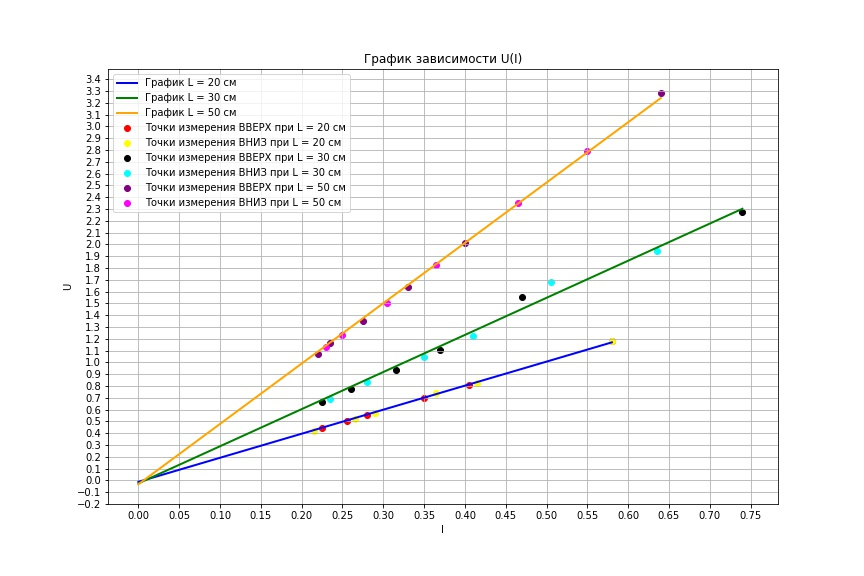
\includegraphics[width=14cm]{schedule}}
\end{center}

%%%Далее снимаем данные сопротивлений пролоки при разных длинах с помощью моста Уитстона, %%%записываем в таблицу.%%%
%%%
%%%По закону Ома $U=RI$ также нужно вспомнить, что погрешность каждого измерения напряжения $\%%%Delta U$ выражается формулой, приложенной в инструкции к вольтметру:%%%
%%%\[\Delta U = (0,003\cdot U + 0,0004)^{3}\]%%%
%%%
%%%Рассчитываем все погрешности напряжения и заносим в таблицу. Также вспоминаем, что погрешность %%%амперметра равна $\Delta I = 0,5 \cdot 5$ мА $= 2,5$ мА -- выражается через класс точности и %%%цену деления.

Чтобы учесть погрешности отдельных измерений напряжения, стоит воспользоваться методом наименьших квадратов.

\[R_{\text{ср}} = \frac{\langle VI \rangle '}{\langle I^2 \rangle '}, \text{ } \sigma_{R_{\text{ср}}} = \frac{1}{\sqrt{N}} \sqrt{\frac{\langle U^2 \rangle '}{\langle I^2 \rangle '} - R^2_{\text{ср}}}\]

Для измеренных данных имеем:
\[R_{\text{ср}1} = 1,986 \text{ Ом, }R_{\text{ср}2} = 3,044\text{ Ом, }R_{\text{ср}3} = 4,979\text{ Ом }\]
\[\sigma_{R_{\text{ср}1}} = 0,009 \text{ Ом, }\sigma_{R_{\text{ср}2}} = 0,036\text{ Ом, }\sigma_{R_{\text{ср}3}} = 0,022\text{ Ом }\]

Данные сопротивлений проволоки, снятые с помощью моста Уитстона, имеют вид:
\[R_{\text{мост}1} = 2,4780 \text{ Ом, }R_{\text{мост}2} = 3,4020\text{ Ом, }R_{\text{мост}3} = 5,3711\text{ Ом }\]

Видим, что данные сопротивлений, снятые с помощью моста и с помощью схемы немного отличаются, так как стоит учитывать влияние человеческого фактора на эксперимент.

В нашем случае $N = 12$ -- число экспериментальных точек. Погрешность амперметра равна
\[\sigma_I = 0,5 \cdot 5 \text{ мА} = 2,5 \text{ мА}\]

В методе наименьших квадратов мы воспользовались погрешностями напряжений, теперь учтём и погрешность амперметра:

\[\sigma_{R_{\text{полн}}} = \sqrt{ \left(\frac{\partial R}{\partial I} \sigma_I\right)^2 + \sigma_{R_{\text{ср}}}^2} = \sqrt{ \left(\frac{R_{\text{ср}}}{I} \sigma_I\right)^2 + \sigma_{R_{\text{ср}}}^2}\]

Для оценки погрешности возьмём предел измерений силы тока $I =$ $0,750$ А.

Отсюда получаем следующие значения погрешностей:
\[\sigma_{R_{\text{полн}1}} = 0,027 \text{ Ом, }\sigma_{R_{\text{полн}2}} = 0,015\text{ Ом, }\sigma_{R_{\text{полн}3}} = 0,014\text{ Ом }\]

Не забываем внести поправку в значения сопротивлений с помощью формулы:

\[R_{\text{пр}} = R_{\text{полн}} (1 + \frac{R_{\text{полн}}}{R_V})\]

Так как поправка очень мала (даже слишком), можно считать, что $R_{\text{пр}} = R_{\text{полн}}$ и $\sigma_{R_{\text{пр}}} = \sigma_{R_{\text{полн}}}$.

Для удобства составим таблицу погрешностей измерения сопротивлений:
\begin{center}
\begin{tabular}{|c|c|c|c|}
\hline 
$L$, см & 20 & 30 & 50 \\ 
\hline 
$R_{\text{полн}}$, Ом & $1,986$ & $3,044$ & $4,979$ \\ 
\hline 
$R_{\text{пр}}$, Ом & $1,986$ & $3,044$ & $4,979$ \\ 
\hline 
$\sigma_{R_{\text{полн}}}$, Ом & $0,027$ & $0,015$ & $0,014$ \\ 
\hline 
$\sigma_{R_{\text{пр}}}$, Ом & $0,027$ & $0,015$ & $0,014$ \\ 
\hline 
$\sigma_{R_{\text{мост}}}$, Ом & $2,4780$ & $3,4020$ & $5,3711$ \\ 
\hline  
\end{tabular} 
\end{center}
\newpage
\begin{center}
 \textbf{Обработка данных для поиска удельного сопротивления проволоки}
\end{center}

Удельное сопротивление проволоки и его погрешность определяются формулами:
\[\rho = \frac{R_{\text{пр}}}{L} \frac{\pi \overline{d_{20}}^2}{4}\]
%%% \text{ } \sigma_{\rho} = \rho \sqrt{\Big( \frac{\sigma_{R_{\text{пр}}}}{R_{\text{пр}}}\Big) ^2 + \Big(\frac{\sigma_S}{S} \Big)^2 + \Big(\frac{\sigma_L}{L} \Big)^2}\]

Здесь $\sigma_{L} = 0,1$ см.
Занесём все результаты в таблицу:
\begin{center}
\begin{tabular}{|c|c|c|c|}
\hline 
$L$, см & 20 & 30 & 50 \\ 
\hline 
$\rho \cdot 10^{-6}$, Ом$\cdot$м & $2,813$ & $1,875$ & $1,125$ \\ 
%%% \hline 
%%% $\sigma_{\rho}\cdot 10^{-6}$, Ом$\cdot$см & $4,93$ & $4,84$ & $4,74$ \\ 
%%% \hline 
\end{tabular} 
\end{center}

\section{Выводы}

В работе получено значение удельного сопротивления образца проволки из нихромового сплава с точностью 


\end{document}